\chapter{\texorpdfstring{From Automata to Nets}{From Automata to Nets}}
\label{ch:08}
\lecturemeta{Lezione 08 \quad\textbullet\quad 2026-07-03 \quad\textbullet\quad Roberto Bruni}{Petri nets basics · Esparza, \emph{Free Choice Petri Nets} (optional)}

Questa lezione dà la \textbf{veste matematica} ai \hyperref[ch:04]{Petri net} che avevamo introdotto in modo intuitivo. Il percorso parte da un modello che probabilmente già conosciamo — gli \textbf{automi a stati finiti} — mostra \emph{perché non bastano} per i sistemi concorrenti, e da lì costruisce i Petri net "deformando" un automa. Lungo la strada fissiamo lo strumento formale che ci serve, i \textbf{multiset}, e diamo la definizione precisa di marcatura, abilitazione, scatto e sequenze di scatto.

Il motivo di tutto questo formalismo è pratico: vogliamo \textbf{analizzare} i processi, non solo disegnarli. L'analisi ha tre facce — la \textbf{validation} (testare la correttezza), la \textbf{verification} (dimostrarla) e la \textbf{performance} (pianificare e ottimizzare) — e i Petri net sono lo strumento giusto perché sono insieme \textbf{visuali, formali e supportati da tool}.

\section{\texorpdfstring{Perché non bastano gli automi}{Perché non bastano gli automi}}

Un \textbf{automa a stati finiti} modella bene i sistemi \textbf{sequenziali}: protocolli, parsing di testo, comportamento di personaggi nei videogiochi, unità di controllo di CPU, distributori automatici, semafori. L'idea è quella di un sistema che si trova, in ogni istante, in \textbf{esattamente uno} stato, e passa da uno stato all'altro leggendo input.

\begin{boxdefinition}{DFA (Deterministic Finite Automaton)}
Un DFA è una tupla $A = (Q, \Sigma, \delta, q_0, F)$ dove: - $Q$ è un insieme finito di \textbf{stati}; - $\Sigma$ è un insieme finito di \textbf{simboli} di input; - $\delta : Q \times \Sigma \to Q$ è la \textbf{funzione di transizione} (dato lo stato corrente e un input, restituisce il prossimo stato); - $q_0 \in Q$ è lo \textbf{stato iniziale}; - $F \subseteq Q$ è l'insieme degli \textbf{stati finali} (accettanti).
\end{boxdefinition}

Un esempio minimo è il \textbf{tornello} (turnstile): è \texttt{locked} finché non si passa una \texttt{card}, che lo porta in \texttt{unlocked}; una \texttt{push} lo riporta in \texttt{locked}.

\begin{center}
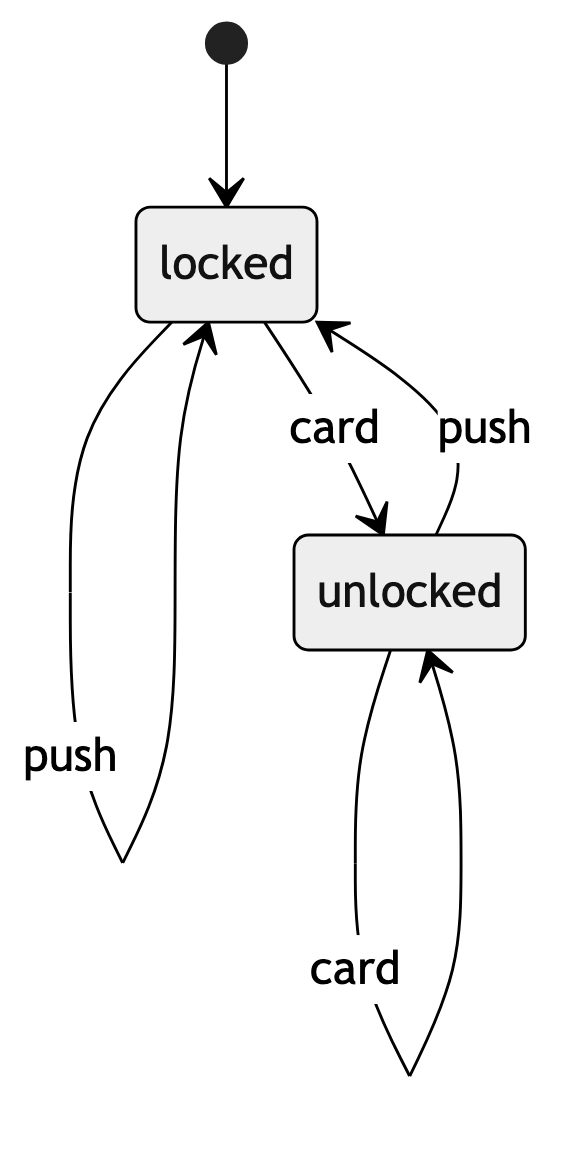
\includegraphics[width=0.36\linewidth,height=0.32\textheight,keepaspectratio]{images/mermaid/08_1.png}
\end{center}

Per descrivere l'effetto di un'\textbf{intera parola} (non un solo simbolo) si estende $\delta$ alla \textbf{funzione destinazione} $\hat\delta : Q \times \Sigma^\star \to Q$, definita per \textbf{induzione} sulla lunghezza della parola:

\[
\hat\delta(q, \epsilon) = q
\]

(parola vuota, si resta fermi), e

\[
\hat\delta(q, wa) = \delta(\hat\delta(q, w), a)
\]

(si processa prima $w$, poi il simbolo finale $a$). Un automa \textbf{accetta} una parola $w$ se $\hat\delta(q_0, w) \in F$, e il suo \textbf{linguaggio} è

\[
L(A) = \{ w \mid \hat\delta(q_0, w) \in F \}
\]

Esiste anche la variante \textbf{non-deterministica} (NFA), in cui $\delta : Q \times \Sigma \to \wp(Q)$ restituisce un \textbf{insieme} di possibili stati successivi (uno stesso input può portare in stati diversi).

\begin{boxwarning}{Il limite degli automi}
Gli automi vanno benissimo per i sistemi \textbf{sequenziali}, ma \textbf{non catturano direttamente il comportamento concorrente}. Se due cose accadono \emph{in parallelo}, un automa è costretto a rappresentarne tutti gli intrecci (interleaving) come stati distinti, con un'esplosione del numero di stati. Un \textbf{Petri net} è per i sistemi \textbf{paralleli e concorrenti} ciò che un automa finito è per i sistemi sequenziali.
\end{boxwarning}

\section{\texorpdfstring{Da un automa a una rete: il "reshaping"}{Da un automa a una rete: il "reshaping"}}

Il modo più illuminante per capire i Petri net è vederli nascere da un automa, con una sequenza di piccole trasformazioni. Partendo da un automa (l'esempio della lezione è un riconoscitore di frasi in linguaggio naturale):

\begin{enumerate}
\item \textbf{Get a token} — si mette un \textbf{gettone} sullo stato iniziale, per segnare "dove siamo".
\item \textbf{Drop the initial-state arrow} — la freccia di start non serve più: lo dice il token.
\item \textbf{Transitions as boxes} — le transizioni (gli archi etichettati) diventano dei \textbf{quadrati} espliciti, nodi a sé stanti.
\item \textbf{Forget final states} — non ci interessa più "accettare" parole, ci interessa l'evoluzione dello stato.
\item \textbf{Add more tokens} — permettiamo \textbf{più di un token} contemporaneamente: ecco la concorrenza.
\item \textbf{Allow for more arcs} — un quadrato può avere più input e più output.
\end{enumerate}

Il risultato ha una nuova terminologia:

\begin{figure}[!htb]
\centering
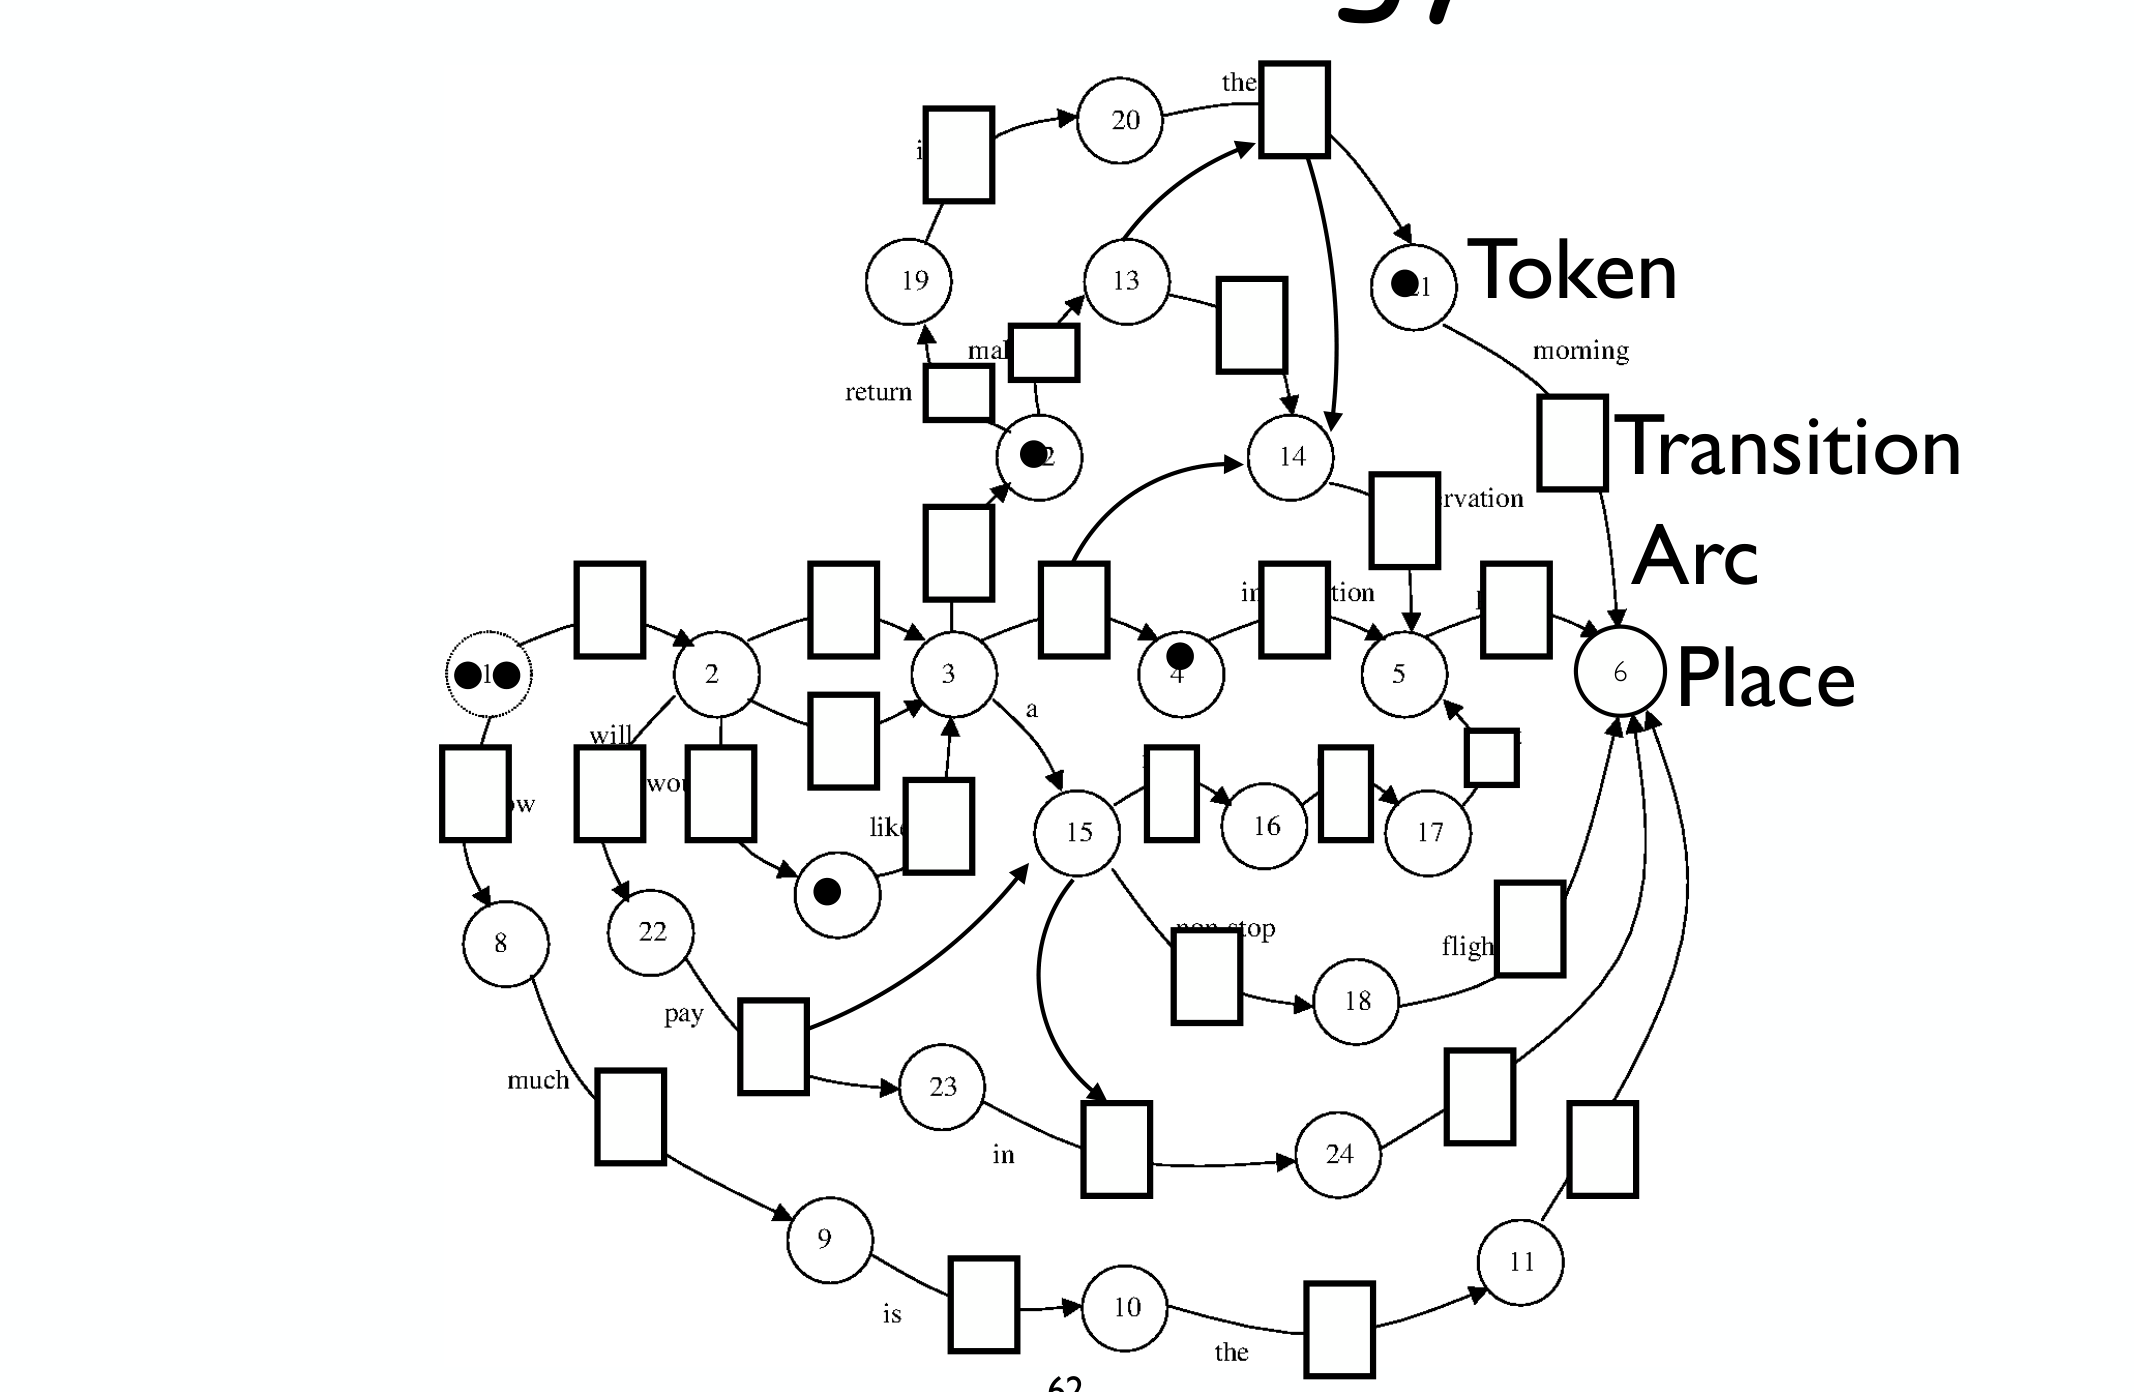
\includegraphics[width=0.74\linewidth,height=0.34\textheight,keepaspectratio]{images/08-nets-intro_p61_reshaping.png}
\caption{L'automa "deformato" in una rete. I nodi-stato diventano \textbf{place} (cerchi), le transizioni etichettate diventano \textbf{transition} (quadrati), i \textbf{token} (pallini) segnano lo stato, e ora possono essercene più d'uno in giro contemporaneamente — è questo a rendere la rete capace di esprimere concorrenza.}
\end{figure}

\begin{boxnote}{I fatti che seguono dalla costruzione}
\begin{itemize}
\item Le reti sono \textbf{grafi bipartiti}: gli archi non collegano mai due place né due transition.
\item Sono una \textbf{struttura statica per un sistema dinamico}: place, transition e archi non cambiano; sono i \textbf{token} a muoversi tra i place.
\item I \textbf{place} sono componenti \textbf{passivi}, le \textbf{transition} componenti \textbf{attivi}.
\item Attenzione: i token \textbf{non fluiscono} lungo gli archi come acqua in un tubo — vengono \textbf{rimossi} dagli input place e \textbf{creati} ex-novo negli output place. È una differenza concettuale importante che spiega perché il numero totale di token può cambiare.
\end{itemize}
\end{boxnote}

\section{\texorpdfstring{Lo strumento formale: i multiset}{Lo strumento formale: i multiset}}

Per descrivere con precisione "quanti token ci sono in ogni place" un insieme ordinario non basta: un place può contenere \textbf{più token uguali}. Serve la nozione di \textbf{multiset} (multiinsieme).

\begin{figure}[!htb]
\centering
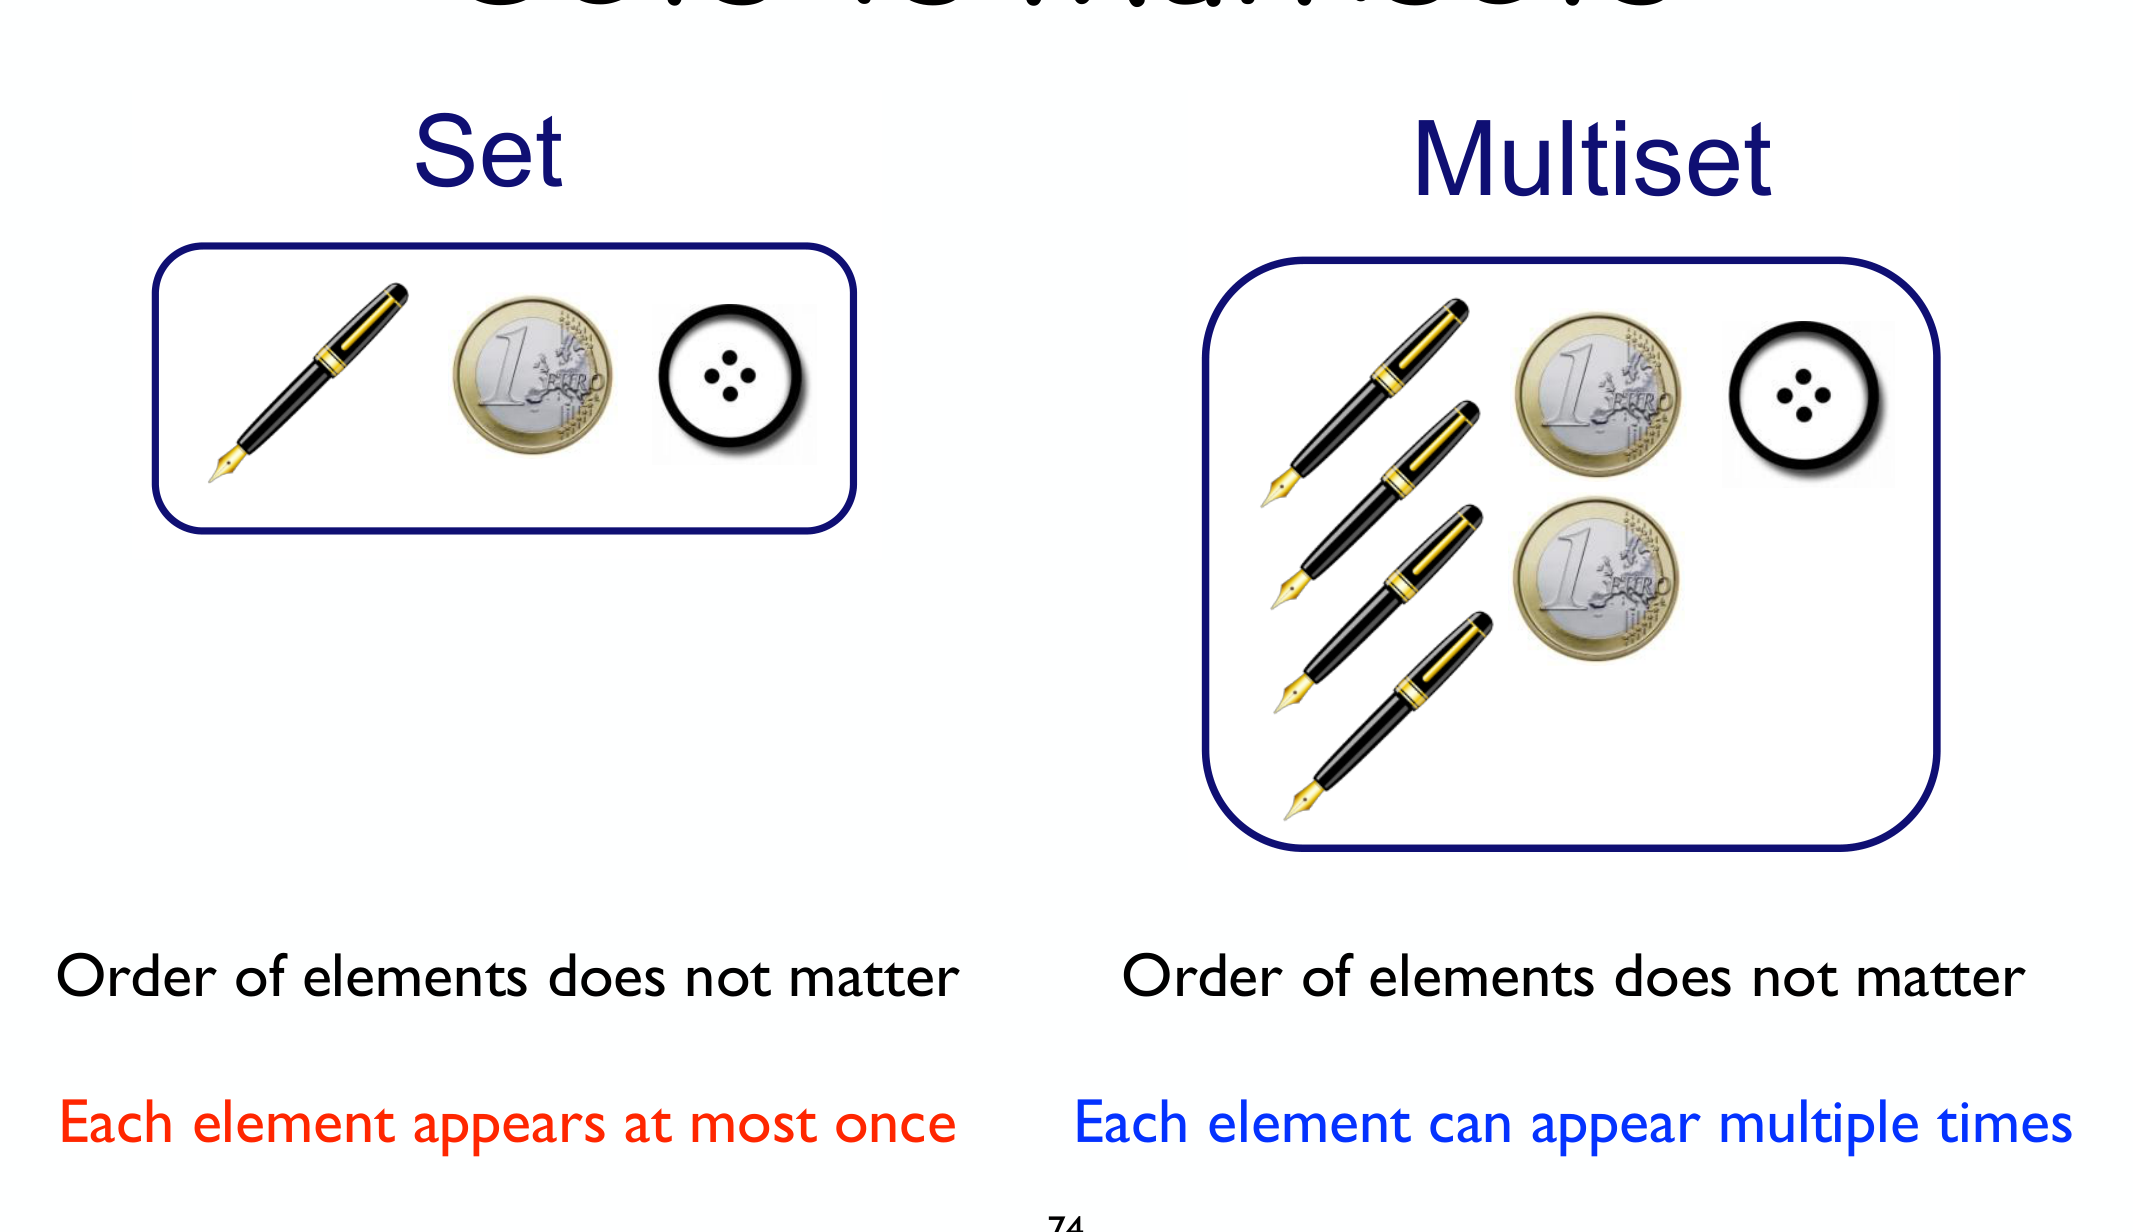
\includegraphics[width=0.74\linewidth,height=0.34\textheight,keepaspectratio]{images/08-nets-intro_p73_sets-vs-multisets.png}
\caption{Set vs multiset. In entrambi l'\textbf{ordine non conta}; la differenza è che in un \textbf{set} ogni elemento compare \textbf{al più una volta}, mentre in un \textbf{multiset} può comparire \textbf{più volte}.}
\end{figure}

\begin{boxdefinition}{Multiset}
Un \textbf{multiset} su un insieme $S$ è una funzione $M : S \to \mathbb{N}$ che a ogni elemento associa la sua \textbf{molteplicità} (quante volte compare). L'insieme dei multiset su $S$ si denota $\mu(S)$ o $S^\oplus$. Diciamo che $x \in M$ se $M(x) > 0$. Un \textbf{set} è il caso particolare in cui ogni molteplicità è 0 oppure 1.
\end{boxdefinition}

Un multiset si scrive comodamente come \textbf{somma formale}:

\[
M = k_1 x_1 + k_2 x_2 + \dots + k_n x_n
\]

dove $k_i$ è la molteplicità di $x_i$ (si omette se vale 1). Per esempio $2a + 3b + c$ è il multiset con due $a$, tre $b$ e una $c$. Le operazioni sono definite molteplicità per molteplicità:

\begin{itemize}
\item \textbf{Contenimento}: \(M \subseteq M' \iff M(x) \le M'(x) \ \text{per ogni } x\)
\item \textbf{Unione (somma)}: \((M + M')(x) = M(x) + M'(x)\)
\item \textbf{Differenza}: \((M - M')(x) = M(x) - M'(x)\), \textbf{definita solo se} $M \supseteq M'$ (altrimenti si andrebbe sotto zero).
\end{itemize}

\begin{boxexample}{Operazioni sui multiset}
\begin{itemize}
\item $3a + 2b \subseteq 2a + 3b + c$? \textbf{No} (serve $3a \le 2a$, falso).
\end{itemize}

\[
(a + 2b) + (2a + c) = 3a + 2b + c
\]

\[
(2a + 3b) - (2a + b) = 2b
\]

\[
(2a + 2b) - (a + c) = \text{non definita}
\]

(manca $c$ nel primo).
\end{boxexample}

\section{\texorpdfstring{Marcatura, abilitazione, scatto (in forma precisa)}{Marcatura, abilitazione, scatto (in forma precisa)}}

Con i multiset possiamo formalizzare tutto ciò che in \hyperref[ch:04]{04 — Petri Nets} avevamo descritto a parole.

\begin{boxdefinition}{Marking (marcatura)}
Una \textbf{marcatura} è un multiset sui place, $M : P \to \mathbb{N}$: dice quanti token stanno in ciascun place. $M(a) = 0$ significa "nessun token in $a$". \textbf{La marcatura è lo stato} del Petri net.
\end{boxdefinition}

\begin{boxdefinition}{Petri net (con marcatura iniziale)}
Un \textbf{Petri net} è una tupla

\[
(P, T, F, M_0)
\]

con $P$ place finiti, $T$ transition finite ($P \cap T = \varnothing$), $F \subseteq (P\times T)\cup(T\times P)$ la flow relation, e $M_0 \in \mu(P)$ la \textbf{marcatura iniziale}. Ricordiamo il \textbf{pre-set} e il \textbf{post-set} di una transizione $t$:

\[
\bullet t = \{p \mid (p,t)\in F\}
\]

\[
t\bullet = \{p \mid (t,p)\in F\}
\]
\end{boxdefinition}

Ed ecco il punto in cui il formalismo dei multiset ripaga: abilitazione e scatto diventano \textbf{operazioni aritmetiche} su marcature.

\begin{boxdefinition}{Enabling e firing (formali)}
\begin{itemize}
\item \textbf{Enabling}: una transizione $t$ è \textbf{abilitata} in $M$ se e solo se
\end{itemize}

\[
\bullet t \subseteq M
\]

cioè se ogni input place ha abbastanza token. Si scrive $M \xrightarrow{t}$ oppure $M[t\rangle$.

\begin{itemize}
\item \textbf{Firing}: una $t$ abilitata in $M$ può \textbf{scattare}, portando alla nuova marcatura
\end{itemize}

\[
M' = M - \bullet t + t\bullet
\]

e si scrive $M \xrightarrow{t} M'$ (o $M[t\rangle M'$). Cioè: \textbf{togli} un token da ogni input place, \textbf{aggiungi} un token in ogni output place.
\end{boxdefinition}

Valgono le stesse osservazioni della lezione 04: lo scatto è \textbf{atomico}, la semantica è \textbf{interleaving} (una transizione alla volta), e il numero totale di token \textbf{può variare} perché $|\bullet t|$ e $|t\bullet|$ possono differire.

Introduciamo anche una notazione compatta per parlare di \emph{esistenza} di mosse:

\[
M \to \quad \text{se qualche transizione è abilitata in } M
\]

\[
M \to M' \quad \text{se } M \xrightarrow{t} M' \text{ per qualche } t
\]

\[
M \centernot{\xrightarrow{t}} \quad \text{se } t \text{ non è abilitata}
\]

\[
M \not\to \quad \text{se nessuna transizione è abilitata (marcatura morta)}
\]

\section{\texorpdfstring{Sequenze di scatto e marcature raggiungibili}{Sequenze di scatto e marcature raggiungibili}}

Un singolo scatto è solo un passo. Ci interessa l'evoluzione completa, cioè le \textbf{sequenze} di scatti.

\begin{boxdefinition}{Firing sequence}
Data una sequenza di transizioni

\[
\sigma = t_1 t_2 \cdots t_{n-1} \in T^\star
\]

scriviamo $M \xrightarrow{\sigma} M'$ se esiste una successione di marcature

\[
M = M_1 \xrightarrow{t_1} M_2 \xrightarrow{t_2} \cdots \xrightarrow{t_{n-1}} M_n = M'
\]

La sequenza può anche essere \textbf{infinita} ($\sigma \in T^\omega$), se il processo non termina mai.
\end{boxdefinition}

\begin{boxdefinition}{Marcature raggiungibili}
Una marcatura $M'$ è \textbf{raggiungibile} da $M$ se $M \xrightarrow{\sigma} M'$ per qualche $\sigma$; si scrive

\[
M \xrightarrow{\;\ast\;} M'
\]

L'insieme di tutte le marcature raggiungibili da $M$ si denota $\text{reach}(M)$ oppure $[M\rangle$.

Nota:

\[
M \xrightarrow{\epsilon} M
\]

ogni marcatura raggiunge sé stessa con la sequenza vuota.
\end{boxdefinition}

Su queste sequenze si definiscono le nozioni di \textbf{concatenazione} (finito + finito = finito; finito + infinito = infinito) e di \textbf{prefisso} ($\sigma_1$ è prefisso di $\sigma$ se $\sigma_1\sigma_2 = \sigma$ per qualche $\sigma_2$). Un fatto utile lega abilitazione e prefissi:

\begin{boxtheorem}{Abilitazione per prefissi}
Una sequenza $\sigma$ è abilitata in $M$ (cioè $M \xrightarrow{\sigma}$) \textbf{se e solo se} \emph{ogni} prefisso $\sigma'$ di $\sigma$ è abilitato in $M$.

\emph{Idea:}

\[
(\Rightarrow) \quad \text{immediato dalla definizione}
\]

\[
(\Leftarrow) \quad \text{se } \sigma \text{ è finita, è banale: è prefisso di sé stessa}
\]

Se invece $\sigma$ è infinita, per ogni $i$ il passo $t_i$ è abilitato perché il prefisso $t_1\cdots t_i$ lo è, e quello è un prefisso finito. $\blacksquare$
\end{boxtheorem}

L'insieme delle marcature raggiungibili $[M_0\rangle$ è il concetto centrale su cui costruiremo l'analisi: rappresenta \textbf{tutti gli stati} in cui il processo può finire. Nella prossima lezione lo organizzeremo in un grafo — l'\textbf{occurrence graph} — per poterlo studiare sistematicamente. $\rightarrow$ \hyperref[ch:09]{09 — Occurrence Graph}